%!TEX root = paper.tex

%\newcommand{\colalg}{{\tt ColAlg}}
%\newcommand{\expthree}{{\tt Exp3}}
%\newcommand{\latentranker}{{\tt LRA}}
%\newcommand{\rowalg}{{\tt RowAlg}}
%\newcommand{\ucb}{{\tt UCB1}}

We propose \emph{latent ranker algorithm ($\latentranker$)} for solving the personalized ranking problem. The pseudocode of $\latentranker$ is in \cref{alg:latent ranker}. $\latentranker$ has two main components, column learning and row ranking.

The column learning algorithm recommends a list of $d$ columns and is the same as in \citet{radlinski2008learning}. But we exploit an additional structure in our problem to show that we learn the optimal columns $J_\ast$. The column learning algorithm are $d$ instances of multi-armed bandit algorithms, which we denote by $\colalg(k)$ for algorithm $k \in [d]$. $\colalg(1)$ learns the most rewarding column on average, $\colalg(2)$ learns the second most rewarding column on average conditioned on the first learned column, as so on.

The row ranking algorithm permutes columns suggested by the column learning algorithm. It consists of multiple instances of full-information algorithms. More precisely, for each user $i \in [K]$ and set of $d$ columns $J$, we have algorithm $\rowalg(i, J)$ with $d!$ arms, which correspond to all possible permutations of $J$. The objective of $\rowalg(i, J)$ is to learn a permutation of $J$ with the highest reward, as measured by \eqref{eq:reward}.

$\latentranker$ interacts with the environment as follows. At time $t$, a random user $i_t$ is revealed to $\latentranker$. Then, in the ascending order of $k \in [d]$, $\colalg(k)$ suggests column $\ell_k$. If $\colalg(k)$ suggests one of the previously suggested columns $\ell_1, \dots, \ell_{k - 1}$, then $\ell_k$ is chosen uniformly at random from the remaining columns. We denote the vector of $d$ suggested columns  by $J_t$. Then $\rowalg(i_t, J_t)$, the row learning algorithm for user $i_t$ and columns $J_t$, selects permutation $\pi_{t, i_t}$ of $J_t$.

The user is recommended a permuted list $\pi_{t, i_t}(J_t)$ and $\latentranker$ observes the individual rewards of all recommended items. Then we update both column and row learning algorithms. The reward of the arm in $\colalg(k)$, which selects the $k$-th column in $J_t$, is updated as follows. If the arm was not one of the previously suggested columns, its reward is $\max \, \{M_t(i_t, J_t(a)): a \in [k]\} - \max \, \{M_t(i_t, J_t(a)): a \in [k - 1]\}$. Otherwise, we update the initially suggested arm with reward $0$. Since $\latentranker$ observes the individual rewards of all recommended items, we can compute the reward of any permutation of $J_t$ in row $i_t$. These rewards are then used to update $\rowalg(i_t, J_t)$. 

%An illustrative diagram of the entire learning process is shown in \cref{fig:rankedbandit}.

%\begin{figure}
%    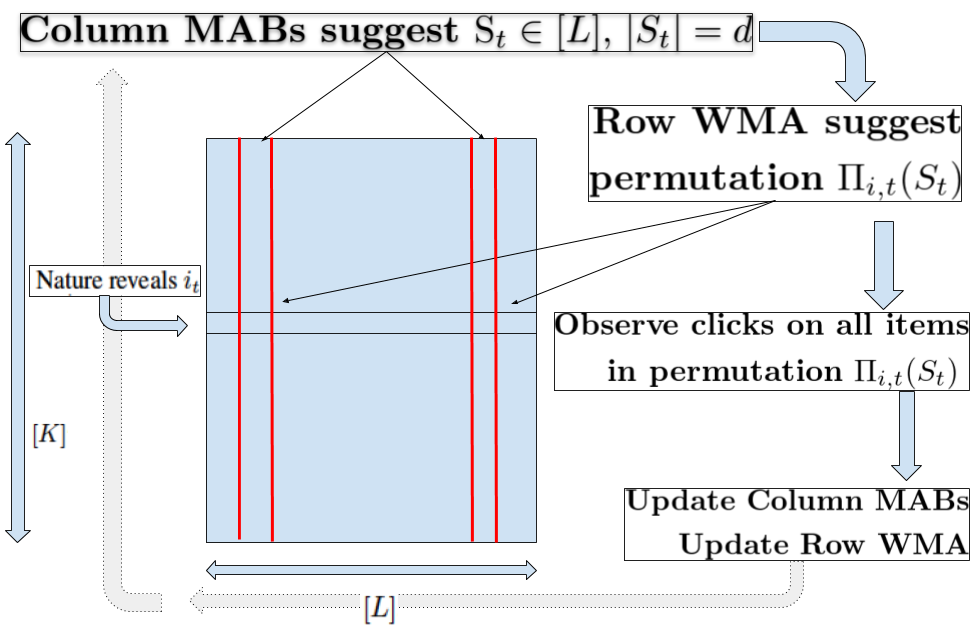
\includegraphics[scale=0.2]{img/RankedBand.png}
%    \caption{Latent Ranked Bandit in rank $d=2$ scenario. \todob{The figure is super confusing. If you want to have it, add a flow chart.}}
%    \label{fig:rankedbandit}
%    \vspace*{-1em}
%\end{figure}

\begin{algorithm}[t]
  \caption{Latent Ranker Algorithm ($\latentranker$)}
  \label{alg:latent ranker}
  \begin{algorithmic}[1]
    \State \textbf{Input:} Rank $d$, horizon $n$
    \State
    \For{$k = 1, \dots, d$}
    \Comment{Initialization}
      \State Initialize $\colalg(k)$
    \EndFor
    \ForAll{$i \in [K], J \subset [L] \text{ such that } |J| = d$}
      \State Initialize $\rowalg(i, J)$
    \EndFor
    \State
    \For{$t = 1, \dots, n$}
      \State User $i_t$ is revealed
      \For{$k = 1, \dots, d$}
      \Comment{Generate response}
        \State $\hat{\ell}_k \gets \text{ Suggested item by } \colalg(k)$
        \If{$\hat{\ell}_k \in \{\ell_1, \dots, \ell_{k - 1}\}$}
          \State $\ell_k \gets$ Random item not in $\{\ell_1, \dots, \ell_{k - 1}\}$
        \Else
          \State $\ell_k \gets \hat{\ell}_k$
        \EndIf
      \EndFor
      \State $J_t \gets (\ell_1, \dots, \ell_d)$
      \State $\pi_{t, i_t} \gets \text{ Suggested permutation by } \rowalg(i_t, J_t)$
      \State
      \State Recommend $\pi_{t, i_t}(J_t)$
      \State Observe $M_t(i_t, J_t(k))$ for all $k \in [d]$
      \State
      \For{$k = 1, \dots, d$}
      \Comment{Update statistics}
        \If{$\ell_k = \hat{\ell}_k$}
          \State Update arm $\ell_k$ of $\colalg(k)$ with reward
          \begin{align*}
            \qquad \quad & \max \, \{M_t(i_t, J_t(a)): a \in [k]\} - {} \\
            & \max \, \{M_t(i_t, J_t(a)): a \in [k - 1]\}
          \end{align*}
        \Else
          \State Update arm $\hat{\ell}_k$ of $\colalg(k)$ with reward $0$
        \EndIf
      \EndFor
      \ForAll{arms $\pi$ in $\rowalg(i_t, J_t)$}
        \State Update arm $\pi$ with reward $r_t(i_t, \pi(J_t))$ in \eqref{eq:reward}
      \EndFor
    \EndFor
  \end{algorithmic}
\end{algorithm}


\subsection{Practical Considerations}
\label{sec:practical considerations}

The proposed $\latentranker$ algorithm only has to update/look through $(Kd + d)$ items for each of the $d$ $\colalg$ and the i-th $\rowalg$ at every timestep $t$. This is in stark contrast to some of the existing matrix completion algorithms which has to reconstruct a $K\times L$ matrix \citep{sen2016contextual} or calculate second or third order tensors \citep{gopalan2016low}. 
%\todob{Discuss time and space complexities of $\latentranker$.}


\todob{Say how we hack $\rowalg$. 
We do not have one row Exp3 for each user and any combination of columns, right? This is how LRA is proposed. This needs to be said.}


Note, that we leave the implementation of the $\colalg$ and $\rowalg$ to the users. For theoretical guarantees we use non-stochastic algorithm $\expthree$ as $\colalg$ and $\WMA$ as $\rowalg$ which will be explained in detail in section \cref{sec:analysis}. For experimental purposes, stochastic algorithms like $\ucb$ or thompson sampling can also be used to improve the performance of $\latentranker$. This has also been explored in \citet{radlinski2008learning} where $\RBA$ uses $\ucb$ for ranking items.

%This is ok. I will write about col Exp3 and row WMA and why they are needed. Great. Also mention that previous works considered UCB1 and we do that as well.

%\todob{Discuss suitable choices for $\colalg$ and $\rowalg$.}
